


\tikzset{every picture/.style={line width=0.75pt}} %set default line width to 0.75pt        

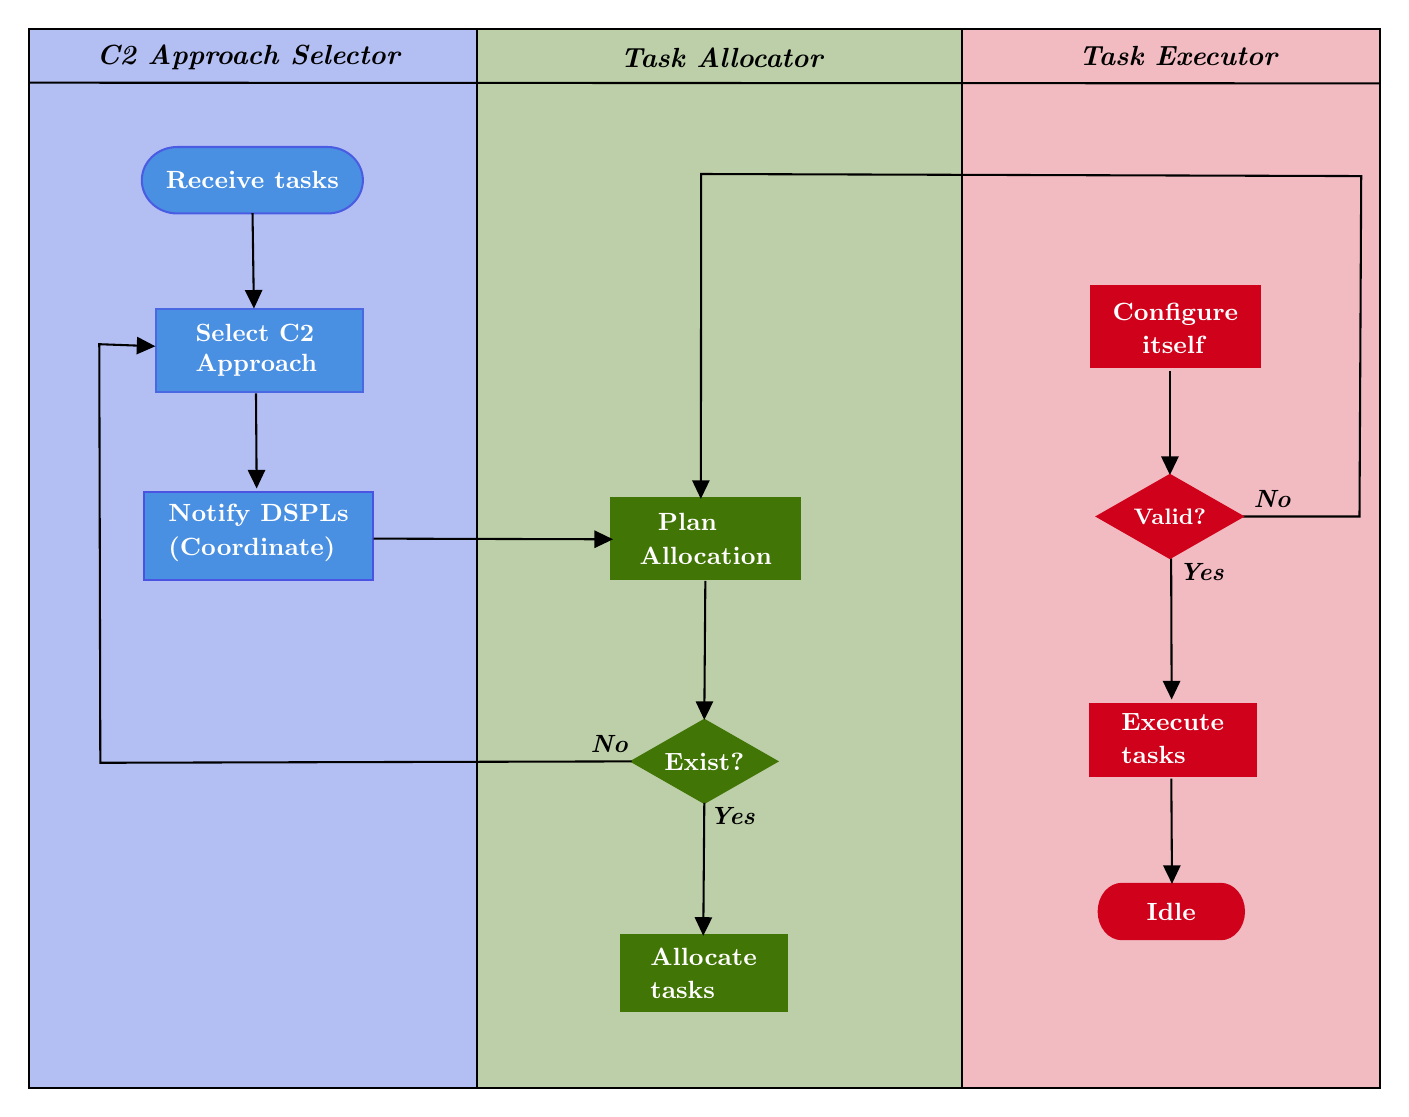
\begin{tikzpicture}[x=0.75pt,y=0.75pt,yscale=-1,xscale=1]
%uncomment if require: \path (0,586); %set diagram left start at 0, and has height of 586

%Shape: Rectangle [id:dp8854253159391561] 
\draw  [fill={rgb, 255:red, 74; green, 102; blue, 226 }  ,fill opacity=0.42 ] (2.5,5) -- (218.5,5) -- (218.5,515.33) -- (2.5,515.33) -- cycle ;
%Shape: Rectangle [id:dp3469463448197052] 
\draw  [fill={rgb, 255:red, 65; green, 117; blue, 5 }  ,fill opacity=0.35 ] (218.5,5) -- (452.33,5) -- (452.33,515.33) -- (218.5,515.33) -- cycle ;
%Shape: Rectangle [id:dp018917795120609204] 
\draw  [fill={rgb, 255:red, 208; green, 2; blue, 27 }  ,fill opacity=0.27 ] (452.33,5) -- (653.5,5) -- (653.5,515.33) -- (452.33,515.33) -- cycle ;
%Straight Lines [id:da8146359528310543] 
\draw    (2.5,31) -- (653,31.33) ;


%Flowchart: Terminator [id:dp16243934787470904] 
\draw  [color={rgb, 255:red, 74; green, 93; blue, 226 }  ,draw opacity=1 ][fill={rgb, 255:red, 74; green, 144; blue, 226 }  ,fill opacity=1 ] (74.04,62) -- (146.46,62) .. controls (155.87,62) and (163.5,69.16) .. (163.5,78) .. controls (163.5,86.84) and (155.87,94) .. (146.46,94) -- (74.04,94) .. controls (64.63,94) and (57,86.84) .. (57,78) .. controls (57,69.16) and (64.63,62) .. (74.04,62) -- cycle ;
%Flowchart: Process [id:dp15412574148578628] 
\draw  [color={rgb, 255:red, 74; green, 104; blue, 226 }  ,draw opacity=1 ][fill={rgb, 255:red, 74; green, 144; blue, 226 }  ,fill opacity=1 ] (64,140) -- (163.5,140) -- (163.5,180) -- (64,180) -- cycle ;
%Flowchart: Process [id:dp48065105856176205] 
\draw  [color={rgb, 255:red, 74; green, 83; blue, 226 }  ,draw opacity=1 ][fill={rgb, 255:red, 74; green, 144; blue, 226 }  ,fill opacity=1 ] (58,228.17) -- (168.5,228.17) -- (168.5,270.83) -- (58,270.83) -- cycle ;
%Flowchart: Process [id:dp6629894570275567] 
\draw  [color={rgb, 255:red, 65; green, 117; blue, 5 }  ,draw opacity=1 ][fill={rgb, 255:red, 65; green, 117; blue, 5 }  ,fill opacity=1 ] (283.17,231.33) -- (374.17,231.33) -- (374.17,270.33) -- (283.17,270.33) -- cycle ;
%Flowchart: Decision [id:dp5160918625824323] 
\draw  [color={rgb, 255:red, 65; green, 117; blue, 5 }  ,draw opacity=1 ][fill={rgb, 255:red, 65; green, 117; blue, 5 }  ,fill opacity=1 ] (328,338) -- (363,358) -- (328,378) -- (293,358) -- cycle ;
%Flowchart: Process [id:dp8044553855974566] 
\draw  [color={rgb, 255:red, 65; green, 117; blue, 5 }  ,draw opacity=1 ][fill={rgb, 255:red, 65; green, 117; blue, 5 }  ,fill opacity=1 ] (287.67,441.67) -- (367.67,441.67) -- (367.67,478.33) -- (287.67,478.33) -- cycle ;
%Straight Lines [id:da6701074801455137] 
\draw    (293,358) -- (37,358.67) -- (36.5,157) -- (61.5,157.93) ;
\draw [shift={(63.5,158)}, rotate = 182.12] [fill={rgb, 255:red, 0; green, 0; blue, 0 }  ][line width=0.75]  [draw opacity=0] (8.93,-4.29) -- (0,0) -- (8.93,4.29) -- cycle    ;

%Straight Lines [id:da6383024146874764] 
\draw    (328,378) -- (327.52,440) ;
\draw [shift={(327.5,442)}, rotate = 270.45] [fill={rgb, 255:red, 0; green, 0; blue, 0 }  ][line width=0.75]  [draw opacity=0] (8.93,-4.29) -- (0,0) -- (8.93,4.29) -- cycle    ;

%Straight Lines [id:da7026427833669057] 
\draw    (328.5,271) -- (328.01,336) ;
\draw [shift={(328,338)}, rotate = 270.43] [fill={rgb, 255:red, 0; green, 0; blue, 0 }  ][line width=0.75]  [draw opacity=0] (8.93,-4.29) -- (0,0) -- (8.93,4.29) -- cycle    ;

%Straight Lines [id:da7965236156041576] 
\draw    (168.67,250.67) -- (282,250.99) ;
\draw [shift={(284,251)}, rotate = 180.17] [fill={rgb, 255:red, 0; green, 0; blue, 0 }  ][line width=0.75]  [draw opacity=0] (8.93,-4.29) -- (0,0) -- (8.93,4.29) -- cycle    ;

%Straight Lines [id:da4788721755855869] 
\draw    (110.33,93.83) -- (110.97,137.83) ;
\draw [shift={(111,139.83)}, rotate = 269.17] [fill={rgb, 255:red, 0; green, 0; blue, 0 }  ][line width=0.75]  [draw opacity=0] (8.93,-4.29) -- (0,0) -- (8.93,4.29) -- cycle    ;

%Straight Lines [id:da7999024493741219] 
\draw    (112,180.67) -- (112.32,224.5) ;
\draw [shift={(112.33,226.5)}, rotate = 269.58] [fill={rgb, 255:red, 0; green, 0; blue, 0 }  ][line width=0.75]  [draw opacity=0] (8.93,-4.29) -- (0,0) -- (8.93,4.29) -- cycle    ;

%Shape: Rectangle [id:dp4479174596462915] 
\draw  [color={rgb, 255:red, 208; green, 2; blue, 27 }  ,draw opacity=1 ][fill={rgb, 255:red, 208; green, 2; blue, 27 }  ,fill opacity=1 ] (514.5,129) -- (595.5,129) -- (595.5,168) -- (514.5,168) -- cycle ;
%Flowchart: Process [id:dp18610523674883006] 
\draw  [color={rgb, 255:red, 208; green, 2; blue, 27 }  ,draw opacity=1 ][fill={rgb, 255:red, 208; green, 2; blue, 27 }  ,fill opacity=1 ] (513.67,330.33) -- (593.67,330.33) -- (593.67,365) -- (513.67,365) -- cycle ;
%Flowchart: Terminator [id:dp6793353293966301] 
\draw  [color={rgb, 255:red, 208; green, 2; blue, 27 }  ,draw opacity=1 ][fill={rgb, 255:red, 208; green, 2; blue, 27 }  ,fill opacity=1 ] (529.2,417) -- (576.8,417) .. controls (582.99,417) and (588,422.97) .. (588,430.33) .. controls (588,437.7) and (582.99,443.67) .. (576.8,443.67) -- (529.2,443.67) .. controls (523.01,443.67) and (518,437.7) .. (518,430.33) .. controls (518,422.97) and (523.01,417) .. (529.2,417) -- cycle ;
%Straight Lines [id:da16428269292090503] 
\draw    (587.33,240) -- (643.67,240) -- (644.5,76) -- (326.5,75) -- (326.34,229.5) ;
\draw [shift={(326.33,231.5)}, rotate = 270.06] [fill={rgb, 255:red, 0; green, 0; blue, 0 }  ][line width=0.75]  [draw opacity=0] (8.93,-4.29) -- (0,0) -- (8.93,4.29) -- cycle    ;

%Straight Lines [id:da6031633731040735] 
\draw    (552.92,260.17) -- (553.16,326.17) ;
\draw [shift={(553.17,328.17)}, rotate = 269.79] [fill={rgb, 255:red, 0; green, 0; blue, 0 }  ][line width=0.75]  [draw opacity=0] (8.93,-4.29) -- (0,0) -- (8.93,4.29) -- cycle    ;

%Straight Lines [id:da15605132192013493] 
\draw    (552.33,170) -- (552.33,218) ;
\draw [shift={(552.33,220)}, rotate = 270] [fill={rgb, 255:red, 0; green, 0; blue, 0 }  ][line width=0.75]  [draw opacity=0] (8.93,-4.29) -- (0,0) -- (8.93,4.29) -- cycle    ;

%Straight Lines [id:da8423233165938356] 
\draw    (553,366.33) -- (553.32,415) ;
\draw [shift={(553.33,417)}, rotate = 269.62] [fill={rgb, 255:red, 0; green, 0; blue, 0 }  ][line width=0.75]  [draw opacity=0] (8.93,-4.29) -- (0,0) -- (8.93,4.29) -- cycle    ;

%Flowchart: Decision [id:dp6377795539825191] 
\draw  [color={rgb, 255:red, 208; green, 2; blue, 27 }  ,draw opacity=1 ][fill={rgb, 255:red, 208; green, 2; blue, 27 }  ,fill opacity=1 ] (552.33,220) -- (587.33,240) -- (552.33,260) -- (517.33,240) -- cycle ;

% Text Node
\draw (109,19) node  [align=left] {\textbf{\textit{C2 Approach Selector}}};
% Text Node
\draw (337,19) node  [align=left] {\textbf{\textit{Task Allocator}}};
% Text Node
\draw (557,18) node  [align=left] {\textbf{\textit{Task Executor}}};
% Text Node
\draw (110.25,78) node  [align=left] {\textbf{{\small \textcolor[rgb]{1,1,1}{Receive tasks}}}};
% Text Node
\draw (113.75,160) node [scale=0.9] [align=left] {\textbf{\textcolor[rgb]{1,1,1}{Select C2 }}\\\textbf{\textcolor[rgb]{1,1,1}{Approach}}};
% Text Node
\draw (113.25,248) node  [align=left] {\textbf{{\small \textcolor[rgb]{1,1,1}{Notify DSPLs}}}\\\textbf{{\small \textcolor[rgb]{1,1,1}{(Coordinate)}}}};
% Text Node
\draw (328.67,250.83) node  [align=left] { \ \ \textbf{{\small \textcolor[rgb]{1,1,1}{ Plan }}}\\\textbf{{\small \textcolor[rgb]{1,1,1}{Allocation}}}};
% Text Node
\draw (328,358) node  [align=left] {\textbf{{\small \textcolor[rgb]{1,1,1}{Exist?}}}};
% Text Node
\draw (327.67,460) node  [align=left] {\textbf{{\small \textcolor[rgb]{1,1,1}{Allocate}}}\\\textbf{{\small \textcolor[rgb]{1,1,1}{ tasks}}}};
% Text Node
\draw (282.67,349.67) node  [align=left] {\textbf{{\small \textit{No}}}};
% Text Node
\draw (342,384.33) node  [align=left] {\textbf{{\small \textit{Yes}}}};
% Text Node
\draw (555,149.5) node  [align=left] {\textcolor[rgb]{1,1,1}{\textbf{{\small Configure}}}\\\textcolor[rgb]{1,1,1}{\textbf{{\small  \ \ \ itself}}}};
% Text Node
\draw (552.33,240) node [scale=0.9,color={rgb, 255:red, 255; green, 255; blue, 255 }  ,opacity=1 ] [align=left] {\textbf{{\small Valid?}}};
% Text Node
\draw (553.67,347) node  [align=left] {{\small \textbf{\textcolor[rgb]{1,1,1}{Execute}}}\\{\small \textbf{\textcolor[rgb]{1,1,1}{ tasks}}}};
% Text Node
\draw (553,430.33) node  [align=left] {{\small \textcolor[rgb]{1,1,1}{\textbf{Idle}}}};
% Text Node
\draw (568,266.67) node  [align=left] {{\small \textbf{\textcolor[rgb]{0,0,0}{\textit{Yes}}}}};
% Text Node
\draw (602,231.33) node  [align=left] {{\small \textbf{\textit{No}}}};


\end{tikzpicture}
